\documentclass[preprint]{article}


% if you need to pass options to natbib, use, e.g.:
%     \PassOptionsToPackage{numbers, compress}{natbib}
% before loading neurips_2023


% ready for submission
\usepackage{neurips_2023}


% to compile a preprint version, e.g., for submission to arXiv, add add the
% [preprint] option:
%     \usepackage[preprint]{neurips_2023}


% to compile a camera-ready version, add the [final] option, e.g.:
%     \usepackage[final]{neurips_2023}


% to avoid loading the natbib package, add option nonatbib:
%    \usepackage[nonatbib]{neurips_2023}


\usepackage[utf8]{inputenc} % allow utf-8 input
\usepackage[T1]{fontenc}    % use 8-bit T1 fonts
\usepackage{hyperref}       % hyperlinks
\usepackage{url}            % simple URL typesetting
\usepackage{booktabs}       % professional-quality tables
\usepackage{amsfonts}       % blackboard math symbols
\usepackage{nicefrac}       % compact symbols for 1/2, etc.
\usepackage{microtype}      % microtypography
\usepackage{xcolor}         % colors
\usepackage{listings}
\usepackage{cite}
\usepackage{graphicx}
\usepackage{hyperref}
\usepackage{amsmath}
\usepackage{algpseudocode}
\usepackage{amsmath}
\usepackage{algorithm}

\lstset{
  breaklines=true,
  basicstyle=\ttfamily\small,
  commentstyle=\color{green!40!black},
  keywordstyle=\color{blue},
  numberstyle=\tiny\color{gray},
  numbers=none,
  frame=single,
  breaklines=true,
  breakatwhitespace=true,
  captionpos=b,
  showstringspaces=false,
  columns=fullflexible,
}

\hypersetup{
    pdftitle={Adapting Safe-for-Work Classifier for Malaysian Language Text: Enhancing Alignment in LLM-Ops Framework},
    pdfauthor={Aisyah Razak, Ariff Nazhan, Ariff Nazhan},
    pdfsubject={Natural Language Processing, Large Language Models, Machine Learning},
    pdfkeywords={language models, malay natural language processing, deep learning},
    colorlinks=true,
    linkcolor=blue,
    citecolor=blue,
    urlcolor=blue
}
\title{Adapting Safe-for-Work Classifier for Malaysian Language Text: Enhancing Alignment in LLM-Ops Framework}
\author{
  Aisyah Razak\thanks{aisyahrazak171@gmail.com} \and
  Ariff Nazhan\thanks{ariffnzhn@gmail.com} \and
  Kamarul Adha\thanks{kamarul.adha360@gmail.com} \and
  Wan Adzhar Faiq Adzlan\thanks{adzhar.faiq@gmail.com} \and
  Mas Aisyah Ahmad\thanks{masaisyahahmad@gmail.com} \and
  Ammar Azman\thanks{dd@gmail.com} \and
}

\begin{document}

\maketitle

\begin{abstract}

\end{abstract}

\section{Introduction}

With the rapid advancements in natural language processing techniques, such as transformer-based architectures, instruction tuning, and reinforcement learning from human feedback, open-domain dialogue systems—commonly known as chatbots or conversational agents—are becoming increasingly prevalent in our daily lives. However, as users, especially children and teenagers, engage with these chatbots, exposure to harmful and provocative text can have significant adverse effects, impacting individuals' mental well-being, relationships, and emotional state. Therefore, ensuring safe and beneficial interactions has become critically important.

The scarcity of data for identifying not safe for work content, particularly in the Malay language, hinders the advancement of undesired content filtration. In this paper, titled \textit{Adapting Safe-for-Work Classifier for Malaysian Language Text: Enhancing Alignment in LLM-Ops Framework}, we address this challenge by initiating the data gathering process to create a comprehensive dataset of harmful texts. Our methodology involves mining data representative of harmful text categories. Our categorization includes the following labels: pornography, harassment, sexist, racist, religious insult, self-harm, psychiatric or mental illness, and safe for work.

We aim to create a robust classifier tailored for Malaysian language text, enhancing the alignment of our large language model operations framework with safety and ethical standards. This classifier serves as a necessary guardrail within the LLM-Ops framework, providing a cost-effective solution for ensuring safe AI. By systematically identifying and filtering out inappropriate content, this classifier will help create a safe and respectful interaction environment for users.

Furthermore, to the best of our knowledge, there is currently no existing local dataset for the Malaysian language that addresses these specific categories of harmful content. Our work thus represents a pioneering effort in developing and applying this crucial safety measure.

\section{Taxonomy}

Designing a universal taxonomy for safe for work guardrails is challenging due to the context-dependent nature of language. Below, we outline our taxonomy for safe-for-work categorization, which will guide the application of guardrails to our large language model or chatbot system. Each category is described to clarify the scope and specifics of what constitutes undesired content:

\begin{itemize}
    \item \textbf{Pornography:} Content that includes explicit sexual descriptions, depictions of sexual acts, or nudity intended to arouse sexual interest. This category covers sexually explicit text, adult content descriptions, and any language or media that depicts sexual activity.

    \item \textbf{Harassment:} Content that targets individuals or groups with the intent to demean, intimidate, or threaten. This includes abusive language, threats, stalking, or any form of verbal harassment aimed at causing emotional or psychological distress.

    \item \textbf{Sexist:} Content that promotes discrimination or prejudice based on gender. This includes sexist remarks, derogatory comments about any gender, and language that reinforces harmful gender stereotypes or inequality.

    \item \textbf{Racist:} Content that discriminates or promotes hatred based on race, ethnicity, or nationality. This includes racial slurs, derogatory remarks about ethnic groups, and any language that supports racial superiority or inferiority.

    \item \textbf{Religious Insult:} Content that disrespects or mocks religious beliefs, practices, or figures. This includes blasphemy, offensive jokes about religions, and language intended to insult or offend individuals based on their religious affiliations.

    \item \textbf{Self-Harm:} Content that depicts or encourages self-injurious behavior or suicide. This includes descriptions of self-harm methods, discussions promoting suicide, and any language that glorifies or encourages self-destructive actions.

    \item \textbf{Psychiatric or Mental Illness:} Content that stigmatizes or discriminates against individuals with mental health conditions. This includes derogatory terms for mental health issues, insensitive jokes, signs of mental distress or illness, and any language that trivializes or mocks mental illness.

    \item \textbf{Safe for Work:} Content that is appropriate for a professional or public environment, free from explicit, offensive, or discriminatory material. This includes clean language, respectful discourse, and content that does not contain any of the above-mentioned undesired elements.
\end{itemize}

This taxonomy will help us systematically identify and filter out inappropriate content, where additional redirection can be made to ensure a safe and respectful interaction environment for users.

\section{Data Source}
The data for this study was collected from various platforms, including social media, public forums, and publicly available datasets. The majority of the data is in the malay language and relevant to the malay context.
By utilizing these comprehensive datasets from multiple sources, we have strengthened the robustness and accuracy of our classification model, enabling it to effectively tackle the challenges of identifying self-harm and sexism in online content.
\subsection{Social Media}
Data was collected from popular social media platforms such as Twitter and Facebook. Two main approaches were employed to gather relevant data:

1. Keyword-based scraping: a list of keywords associated with explicit content was compiled. These keywords were used to extract tweets from the platform.

2. Profile-based scraping: a list of profiles known for regularly posting NSFW content was curated. Posts from these profiles were then scraped to obtain a more targeted dataset.

The combination of these two scraping methods resulted in a comprehensive and diverse dataset from social media, capturing both keyword-specific content and data from profiles that frequently share explicit material.


\subsection{Public Articles}

For public articles, we have collected data from various articles and blogs which are \href{http://b.cari.com.my}{b.cari}, which hosts a wide range of user-generated content in Malay.

The collected dataset consists of human dialogues extracted from these articles and blog posts. It notably includes some dialogues that contain nsfw content. The inclusion of such dialogues, while potentially controversial, is important to allow the trained classifier to effectively detect explicit content that may realistically occur in open-ended dialogue systems.

\subsection{Public Datasets}

We have also collected data from publicly available dataset on kaggle such as \href{https://www.kaggle.com/datasets/nikhileswarkomati/suicide-watch}{Kaggle: Suicide and Depression Detection} datasets. The dataset is a collection of posts from the "SuicideWatch" and "depression" subreddits of the Reddit platform. This dataset contains a wide range of suicide ideation contexts, providing valuable insights for our research.

We also leverage \href{https://github.com/rewire-online/edos}{Explainable Detection of Online Sexism (EDOS)} from github and \href{http://nlp.uned.es/exist2021/}{EXIST: sEXism Identification in Social neTwork (EXIST)} from web that contain a diverse collection of sexism statements, which have significantly contributed to the success of our classifier in identifying and categorizing such content.

\section{Methodology}

Supervised text classification requires reliable class labels for training data. However, obtaining these labels can be complex and expensive. Typically, labels are added sequentially by querying an annotator until satisfactory performance is achieved. We introduced an approach that leverages active learning, knowledge distillation of large language models, and text clustering to reduce annotation effort and construct a collection of labeled not safe for work (NSFW) data from our gathered data.

Following figure illustrates the overall flow employed in our methodology to collect NSFW dataset aims to label malaysian dataset for alignment in LLMOps framework.


\subsection{Knowledge Distillation of Large Language Models}

Data annotation using knowledge distillation from a large language model (LLM) involves prompting a teacher LLM to generate a label \( y \) for a given input \( x \) as the foundational knowledge. This paper primarily explores the zero-shot paradigm, where the LLM receives only the input \( x \) and an instruction \( I \) without any labeled examples or demonstrations. This straightforward yet effective method of extracting knowledge from teacher LLMs has been widely applied to various tasks and applications. It only requires an input dataset, which is then processed by the LLM to produce the desired label \( y \).

In this annotation stage, we utilized two different large language models: mistral-7b and mallam-small. By leveraging mistral-7b, which excels with English-centric prompts, we translated our scraped data into English to provide better context and achieve reliable outputs from the model. While for mallam, we provided inputs from the original malay text as it has better contextual meaning compared to the other models. Below is the prompt we used to generate the labels from the models:

\begin{lstlisting}[breaklines=true]

    text: <text content>

    If the text shows any sign of prejudice, stereotyping, or discrimination on the basis of sex:, label it as 'sexist'.
    If the text shows any sign of content that threatens, incites, glorifies, or expresses desire for violence or harm., label it as 'violence'.
    If the text shows any sign of prejudice, discrimination, or antagonism by an individual, community, or institution against a person or people on the basis of their membership of a particular racial or ethnic group, label it as 'racist'.
    If the text shows any sign of content depicting adult nudity or sexual behavior that is pornographic or intended to cause sexual arousal, label it as 'porn'.
    If the text shows any sign of psychiatric or mental illness, label it as 'psychiatric or mental illness'.
    If the text shows any sign of promotion, or otherwise encourage, suicide or self-harm, label it as 'self-harm'.
    If the text shows any sign of harassment, label it as 'harassment'.
    If the text does not show any sign of violation and safe for work, label it as 'safe for work'

    Only use the label from above choice.

    return the result in JSON format {'label', 'explain'}

\end{lstlisting}


\subsection{Centroid Based Filtering}

We utilize labeled data obtained from a large language model (LLM) to enhance the quality and consistency of our dataset. First, we compute the centroid of the feature vectors for the labeled data, representing the central point in the feature space. The determination of similarity is guided by the Euclidean distance formula, where lower values indicate greater similarity and higher values signify greater dissimilarity. 

By measuring the distance of each data point from this centroid, we can identify and filter out data points that are far from the centroid. These distant points are likely to be outliers or less representative of the core topic data distribution. This ensures that the labels encapsulate the nuanced semantics of the specific topic. This filtering process enhances the dataset by retaining data that is more coherent and relevant, thereby improving the performance of the classifier.


\begin{figure}[h]
  \centering
  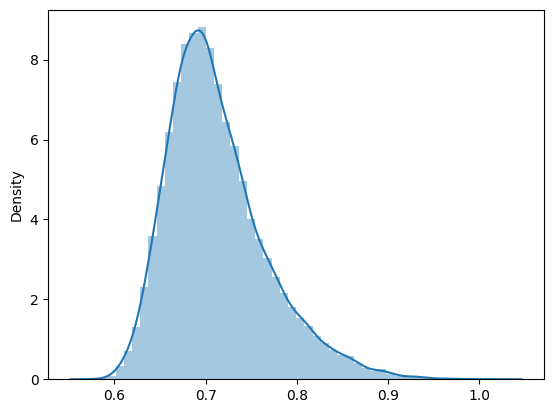
\includegraphics[width=0.6\linewidth]{img/centroid-distance.png}
\end{figure}

\subsection{Active Learning}

We use relevant data from a specific category to train a classifier model. The trained model is then used to classify unlabeled data, a process known as pseudolabeling. The outputs given by the classifier are reviewed before feeding all the unlabeled data into a larger classifier model. This iterative process continues until the desired accuracy is achieved.

The following algorithm outlines the active learning process:

\begin{algorithm}[H]
\caption{Active Learning for Single Label Classifier}
\begin{algorithmic}[1]
\State \textbf{Input:} Labeled data \(D_L\), Unlabeled data \(D_U\), Classifier model \(M\), Desired accuracy \(A_{desired}\)
\State \textbf{Output:} Trained classifier model \(M\)

\While {Accuracy \(A\) < \(A_{desired}\)}
    \State Train classifier \(M\) on \(D_L\)
    \State Predict labels for \(D_U\) using \(M\) (pseudolabeling)
    \State Filter high-confidence predictions from \(D_U\) to create a new labeled dataset \(D_{L_{new}}\)
    \State Update labeled dataset: \(D_L \leftarrow D_L \cup D_{L_{new}}\)
    \State Retrain classifier \(M\) on the updated \(D_L\)
    \State Manually evaluate the accuracy \(A\) of \(M\)
\EndWhile

\State \textbf{return} Trained classifier model \(M\)
\end{algorithmic}
\end{algorithm}



\section{Evaluation}


\section{Acknowledgement}

Special thanks to Malaysia-AI volunteers especially \href{https://www.linkedin.com/in/ammar-azman/}{Ammar Azman}, \href{https://www.linkedin.com/in/amzar96/}{M. Amzar}, \href{https://www.linkedin.com/in/muhammad-farhan-helmy-0529501a7/}{Muhammad Farhan}, \href{https://www.linkedin.com/in/syafie-nizam/}{Syafie Nizam}, \href{https://www.linkedin.com/in/alif-aiman-1b334b24b/}{Alif Aiman}, \href{https://www.linkedin.com/in/azwan-zuharimi/}{Azwan Zuharimi} and \href{https://www.linkedin.com/in/haziqzikry/}{Haziq Zikry} for contributing dataset to train Malaysian Reranker models.

We would like to express our gratitude to NVIDIA Inception for generously providing us with the opportunity to train our model on the Azure cloud. Their support has played a crucial role in the success of our research, enabling us to leverage advanced technologies and computational resources.

We extend our thanks to the wider research community for their valuable insights and collaborative discussions, which have greatly influenced our work. This paper reflects the collective efforts and contributions from both NVIDIA Inception and the broader research community.

\section{Conclusion}

\bibliography{neurips_2023}{}
\bibliographystyle{unsrt}

\end{document}